% Bismillahi-r-Rahmani-r-Rahim
% In the Name of God the Merciful, the Compassionate

\documentclass[preprint,leqno]{elsarticle}
%\documentclass{article}

\author{Daoud Clarke}
\date{\today}
\title{Riesz Logic}

%\usepackage{times}
%\usepackage{mathptmx}
%\usepackage{newtxtext,newtxmath}

\usepackage{amsmath}
\usepackage{stmaryrd}
\usepackage{cmll}
\usepackage{graphicx}
\usepackage{caption}
\usepackage{subcaption}
%\usepackage{mathabx}

\newdefinition{definition}{Definition}
\newproof{proof}{Proof}

%\newcommand{\interp}[1]{\ldbrack #1 \rdbrack}
\newcommand{\interp}[1]{\llbracket #1 \rrbracket}

\begin{document}


\begin{abstract}
We introduce Riesz Logic, whose models are lattice ordered groups,
which generalise Riesz spaces (vector lattices), and show soundness
and completeness. Our motivation is to provide a logic for
distributional semantics of natural language, where words are
typically represented as elements of a vector space whose dimensions
correspond to contexts in which words may occur. This basis provides a
lattice ordering on the space, and this ordering may be interpreted as
``distributional entailment''. Several axioms of Riesz Logic are
familiar from Basic Fuzzy Logic, and we show how the models of these
two logics may be related; Riesz Logic may thus be considered a new
fuzzy logic.
\end{abstract}

\maketitle


\section{Introduction}

Much of the original motivation for fuzzy logic revolved around
linguistic intuitions, for example the notion that ``tall'' is not a
black and white concept, but that there are degrees of
tallness. Indeed, one of the proposed applications for these ideas was
in linguistics \cite{Zadeh:73}. However, these ideas were never
directly adopted by the linguistics or computational linguistics
community. Instead, fuzziness has crept into natural language
semantics by the widespread adoption of ``distributional semantics'',
in which the meaning of words is determined by the contexts in which
they occur. This idea has its origin in the work of Firth
\cite{Firth:57} and Harris \cite{Harris:68}, and the philosophy of
Wittgenstein \cite{Wittgenstein:53}.


We introduce Riesz Logic (RL), a variant of fuzzy logic whose models
are abelian lattice ordered groups, of which the most familiar
examples are vector lattices, or Riesz spaces.
% Our logic has axioms very similar to those
% of fuzzy logics, in particular Basic Fuzzy Logic (BL), although the
% models are quite different.
%

% % These two together allow proof of first five BAL axioms
% P((x => y) => ((y => z) => (x => z)))         # label(R1).
% P(((y => z) => (x => z)) => (x => y))         # label(R2).

% % Needed to prove BALPI and BALPa
% P(x => x v y)                                 # label(R3).

% % Needed to prove BALO
% P(x v y => y v x)                             # label(R4).

% %% % Adapted from BALP
% P((x v y) v y => x v y)                       # label(R5).

% % Definition of zero
% P(0 => (z => z))                              # label(R6a).
% P((z => z) => 0)                              # label(R6b).

% %% % Adapted from BALO
% P(((x => y) v 0 => (y => x) v 0) => (y => x)) # label(R7a).
% P((y => x) => ((x => y) v 0 => (y => x) v 0)) # label(R7b).

%
RL has the following inference rules:\\
\begin{minipage}{0.49\textwidth}
\begin{gather}
  \tag{MP} \frac{\phi, \phi \rightarrow \psi}{\psi}
\end{gather}
\end{minipage}
\begin{minipage}{0.49\textwidth}
\begin{gather}
  \tag{RI} \frac{\phi \rightarrow \psi}{\phi \lor \chi \rightarrow \psi \lor \chi}
\end{gather}
\end{minipage}
\vspace{0.3cm}\\
and the following axioms:
\begin{align}
  \tag{R1a} &(\phi \rightarrow \psi) \rightarrow ((\psi \rightarrow \chi)
  \rightarrow (\phi \rightarrow \chi))\\
  \tag{R1b} &((\psi \rightarrow \chi) \rightarrow (\phi \rightarrow
  \chi)) \rightarrow (\phi \rightarrow \psi)\\
  \tag{R2} &\phi \rightarrow \phi \lor \psi\\
  \tag{R3} &\phi \lor \psi \rightarrow \psi \lor \phi,\\
  \tag{R4} &(\phi \lor \psi)\lor \psi \rightarrow \phi \lor \psi\\
  \tag{R5a} &0 \rightarrow (\phi \rightarrow \phi)\\
  \tag{R5b} &(\phi \rightarrow\phi) \rightarrow 0\\
  \tag{R6a} &((\phi \rightarrow \psi)\lor 0 \rightarrow (\psi \rightarrow \phi) \lor 0) \rightarrow (\psi \rightarrow \phi)\\
  \tag{R6b} & (\psi \rightarrow \phi) \rightarrow ((\phi \rightarrow \psi)\lor 0 \rightarrow (\psi \rightarrow \phi) \lor 0)
\end{align}
In this paper we prove the soundness and completeness of this logic
with respect to abelian lattice ordered groups, with formulas
interpreted as asserting positivity. In doing this, we relate RL to
the Logic of Equilibrium, known as BAL \cite{Galli:04}.

%  In particular there is no ``True'' or
% ``False'' constant, instead there is a zero value which indicates
% maximal uncertainty about a proposition. We demonstrate that our logic
% is equivalent to the logic BAL of

\section{Motivation}


\section{Relation to Fuzzy Logic}

\begin{figure}
  \begin{subfigure}{0.49\textwidth}
    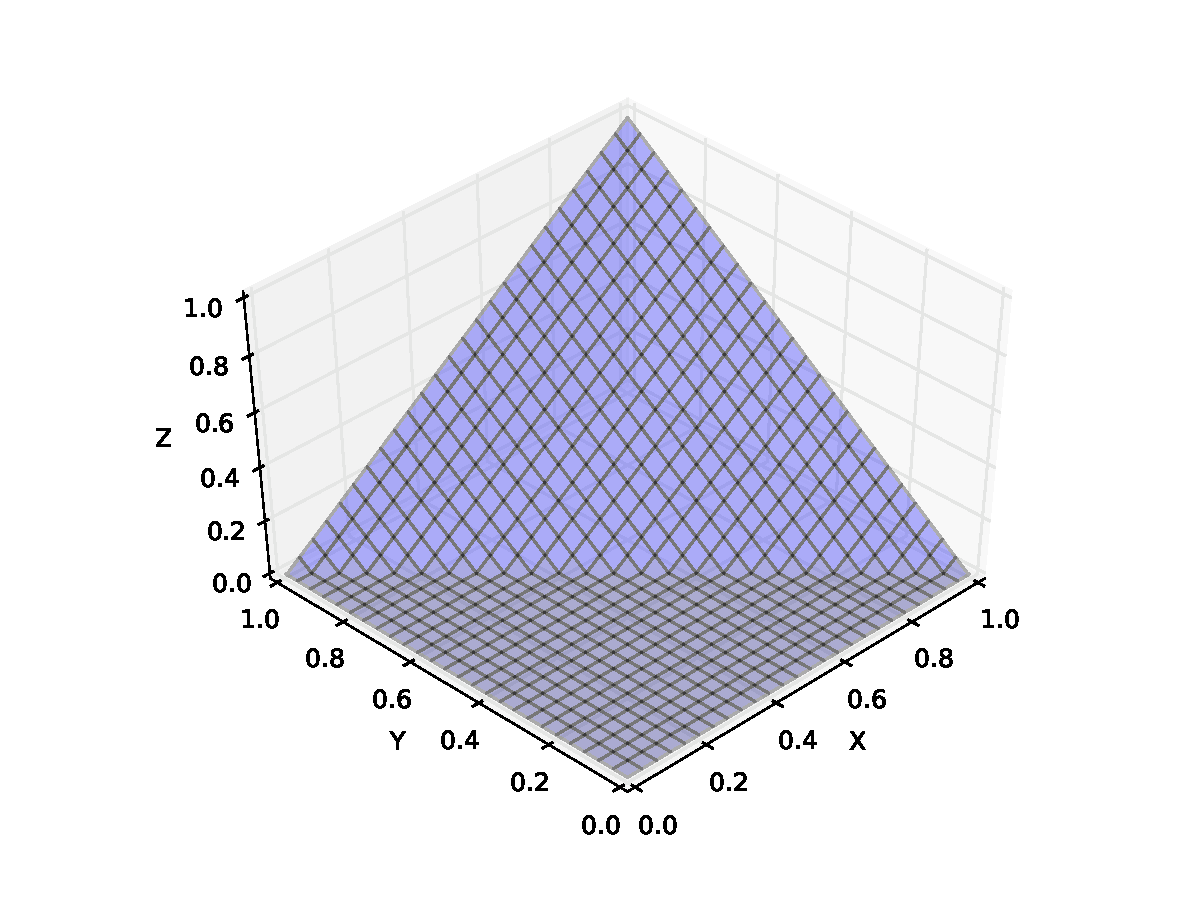
\includegraphics[width=\textwidth]{lukasiewicz.pdf}
    \caption{\L ukasiewicz t-norm}
    \label{fig:lukasiewicz}
  \end{subfigure}
  \begin{subfigure}{0.49\textwidth}
    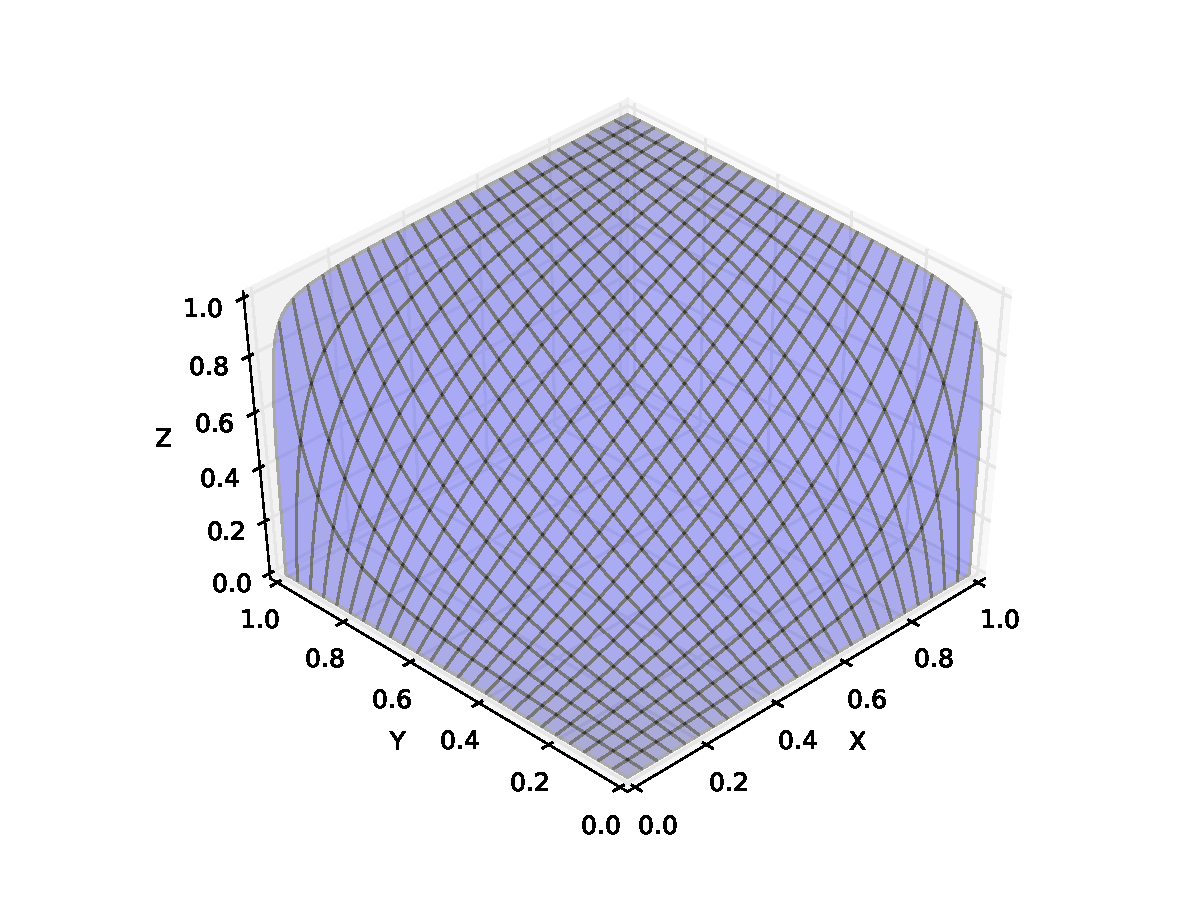
\includegraphics[width=\textwidth]{rieszfunc.pdf}
    \caption{Logistic addition}
    \label{fig:logistic}
  \end{subfigure}
  \caption{Mapping real numbers to the interval $[0,1]$ gives a new
    operation corresponding to addition (\subref{fig:logistic}), which
    bears some similarities to t-norms (\subref{fig:lukasiewicz}).}
\end{figure}

\section{Interpretations}

We prove the soundness and completeness of RL with respect to
abelian lattice ordered groups.

\begin{definition}[Lattice Ordered Group]
  A partially ordered group is a tuple $\langle G, +, \le\rangle$ such
  that $\langle G, +\rangle$ is a group, and $\le$ is a partial order
  on $G$ such that if $u \le v$ then $u + w \le v + w$ and $w + u \le
  w + v$. If $\le$ is a lattice order, then $G$ is called a lattice
  ordered group. Where there is no confusion, we refer to the lattice
  ordered group $\langle G, +, \le\rangle$ as simply $G$. We denote
  the lattice meet and join by $\land$ and $\lor$ respectively.

  The \textbf{positive part} of $u\in G$ is written $u^+$ and is defined
  as $u^+ = u\lor 0$; its \textbf{negative part} is defined as $u^- =
  (-u)\lor 0$.
\end{definition}

Riesz spaces are abelian lattice ordered groups where the group
operation is vector space addition, and the vector space zero is the
unit of the group.

An interpretation $\langle G, F\rangle$ for RL is an abelian lattice
ordered group $G$ and a function $F$ that maps variables in RL to
elements of $G$. A formula $x$ has the interpretation $\interp{x}$
defined recursively as follows:
\begin{itemize}
\item $\interp{\phi} = F(\phi)$
\item $\interp{x \rightarrow y} = \interp{y} - \interp{x}$
\item $\interp{x \lor y} = \interp{x} \lor \interp{y}$
\end{itemize}
The formula $x$ is interpreted as asserting that $0 \le
\interp{x}$. Thus, for example, the formula $\phi \rightarrow \psi$ is
interpreted as the assertion $0 \le F(\psi) - F(\phi)$, or $F(\phi)
\le F(\psi)$. A formula $x$ is satisfiable if there is some
interpretation such that $0 \le \interp{x}$; it is a theorem or
tautology if $0 \le \interp{x}$ for all interpretations.

\section{Soundness}

Proving soundness of the logic amounts to proving the validity of the
rule and axioms.

%\subsection{Modus Ponens}

\begin{proof}[Modus Ponens]
If $0 \le F(\phi)$ and $0 \le F(\psi) - F(\phi)$ then
$0 \le F(\psi)$ by transitivity of $\le$.
\end{proof}

\begin{proof}[R1]
  Since R1a is the converse of R1b, they may be taken together as
  asserting equality, by the antisymmetry of $\le$. Thus we need to
  show:
  \begin{align*}
    \interp{\phi \rightarrow \psi} & = \interp{(\psi \rightarrow
      \chi) \rightarrow (\phi \rightarrow \chi)}\\
    F(\psi) - F(\phi) & = \interp{\phi \rightarrow \chi} -
    \interp{\psi \rightarrow \chi}\\
    & = F(\chi) - F(\phi) - F(\chi) + F(\psi)\\
    & = F(\psi) - F(\phi).
  \end{align*}
\end{proof}
R2--4 are trivially seen to be properties of the partial ordering. R5
defines the symbol 0 such that $\interp{0}$ is the identity of the
group, which we also denote 0.

\begin{proof}[R6]
\begin{align*}
  \interp{(\phi \rightarrow \psi)\lor 0 \rightarrow (\psi \rightarrow \phi) \lor 0} &= \interp{\psi \rightarrow \phi}\\
  \interp{(\psi \rightarrow \phi) \lor 0} - \interp{(\phi \rightarrow \psi)\lor 0} &= F(\phi) - F(\psi)\\
  (F(\phi) - F(\psi))^+ - (F(\phi) - F(\psi))^- & =F(\phi) - F(\psi)
\end{align*}
%% where $x^+ = x\lor 0$ and $x^- = (-x)\lor 0$ are the positive and
%% negative parts of $x$ respectively.
The identity $x = x^+ - x^-$ is
well known for lattice ordered groups, and can be shown by $x + x^- =
x + (-x)\lor 0 = (x - x)\lor(x + 0) = 0\lor x = x^+$.
\end{proof}

\section{Completeness}

We show completeness by relating RL to BAL \cite{Galli:04}. The
semantics of BAL is also lattice ordered groups, but a statement is
interpreted as stating equality with zero. BAL has the primitive
binary operation $\rightarrow$ and unary operation ${}^+$. The former
is interpreted as in RL and the latter has the interpretation
$\interp{x^+} = \interp{x}^+$, i.e.~it maps elements to their positive
parts. Thus the statement $\phi \rightarrow \psi$ in BAL is
interpreted as an assertion that $F(\psi) - F(\phi) = 0$ or $F(\phi) =
F(\psi)$. The logic has the following axioms:
\begin{align}
  \tag{BALB} &(\phi \rightarrow \psi) \rightarrow ((\chi \rightarrow \phi)
  \rightarrow (\chi \rightarrow \psi))\\
  \tag{BALC} &(\phi \rightarrow (\psi \rightarrow \chi)) \rightarrow
  (\psi \rightarrow (\phi \rightarrow \chi))\\
  \tag{BALN} &((\phi \rightarrow \psi) \rightarrow \psi) \rightarrow
  \phi\\
  \tag{BALP} &\phi^{++} \rightarrow\phi^+\\
  \tag{BALO} &((\psi\rightarrow\phi)^+
  \rightarrow(\phi\rightarrow\psi)^+)\rightarrow
  (\phi\rightarrow\psi)
\end{align}
and the following inference rules:\\
\begin{minipage}{0.49\textwidth}
\begin{gather}
  \tag{BALMP} \frac{\phi, \phi \rightarrow \psi}{\psi},\\
  \tag{BALPI} \frac{\phi}{\phi^+},
\end{gather}
\end{minipage}
\begin{minipage}{0.49\textwidth}
\begin{gather}
  \tag{BALG} \frac{\phi, \psi}{\phi \rightarrow \psi},\\
  \tag{BALMI} \frac{(\phi\rightarrow\psi)^+}{(\phi^+\rightarrow\psi^+)^+}.
\end{gather}
\end{minipage}
\vspace{0.3cm}\\
Note that BAL has the same expressive power as RL: a statement $x$ in
the Logic of Equilibrium is equivalent to two statements, $x$ and
$x\rightarrow 0$ in Riesz Logic. Conversely, the statement $x$ in
Riesz Logic is equivalent to the statement $(x\rightarrow 0)^+$ in the
Logic of Equilibrium: this is asserting that the negative part of $x$
is zero, which is the same as asserting that $x$ itself is positive.

Another consequence of the difference in interpretation between the
two logics is that it is not enough to show that every tautology in
BAL is a tautology in RL; we also expect their converses to hold. Our
proof of completeness is thus in three parts:
\begin{itemize}
  \item We show that the inference rules of BAL are valid in RL;
  \item We show that the axioms of BAL and their converses are
    tautologies of RL;
  \item We show that for every tautology in BAL of the form
    $(x\rightarrow 0)^+$, there is a tautology $x$ in RL.
\end{itemize}

\subsection{Inference Rules}

Premises in BAL inference rules are stronger statements than in RL
since they are interpreted as asserting equality. Similarly, we need
to deduce two conclusions in RL for each conclusion in a BAL inference
rule in order to assert equality in RL. Specifically, given a BAL
inference rule
$$\frac{\phi_1,\phi_2,\ldots}{\psi},$$
we need the following inference rules in RL:
$$\frac{\phi_1,\phi_2,\ldots, \phi_1\rightarrow 0, \phi_2\rightarrow
  0, \ldots}{\psi}\text{ and }\frac{\phi_1,\phi_2,\ldots,
  \phi_1\rightarrow 0, \phi_2\rightarrow 0, \ldots}{\psi \rightarrow
  0}.$$
For each rule BALR in BAL, we will refer to these two versions as
BALR+ and BALR$-$ respectively.

\begin{proof}[BALMP]
BALMP+ follows trivially from the assumption of the rule MP in RL. To see BALMP$-$:
\begin{align}
\tag{1} & \alpha \rightarrow 0 & \text{(assumption)}\\
\tag{2} & (\alpha \rightarrow \beta) \rightarrow 0 & \text{(assumption)}\\
\tag{3} & (((\phi \rightarrow \psi) \rightarrow (\chi \rightarrow \psi)) \rightarrow \omega) \rightarrow ((\chi \rightarrow \phi) \rightarrow \omega) & \text{(MP, R1a, R1a)}\\
\tag{4} & \phi \rightarrow ((\phi \rightarrow \psi) \rightarrow \psi) & \text{(MP, R1b, R1b)}\\
\tag{5} & (0 \rightarrow \phi) \rightarrow ((\alpha \rightarrow \beta) \rightarrow \phi) & \text{(MP, 2, R1a)}\\
\tag{6} & ((\alpha \rightarrow 0) \rightarrow \phi) \rightarrow \phi & \text{(MP, 1, 4)}\\
\tag{7} & (\phi \rightarrow \alpha) \rightarrow (\phi \rightarrow 0) & \text{(MP, 6, 3)}\\
\tag{8} & (\alpha \rightarrow \beta) \rightarrow (\phi \rightarrow \phi) & \text{(MP, R5a, 5)}\\
\tag{9} & \beta \rightarrow \alpha & \text{(MP, 8, R1b)}\\
\tag{10} & \beta \rightarrow 0 & \text{(MP, 9, 7)}

\end{align}
\end{proof}

\begin{proof}[BALPI]
BALPI+ follows from R2. To see BALPI$-$:
\begin{align*}
1. & \alpha \rightarrow 0 \hfill \text{by assumption}\\
2. & \phi \rightarrow ((\phi \rightarrow \psi) \rightarrow \psi) \hfill \text{by MP, R1b, R1b}\\
3. & \phi \lor \psi \rightarrow (\phi \lor \chi) \lor \psi \hfill \text{by RI, R2}\\
4. & (\phi \lor \psi) \lor \chi \rightarrow (\psi \lor \phi) \lor \chi \hfill \text{by RI, R3}\\
5. & (\phi \lor \psi \rightarrow \chi) \rightarrow (\psi \lor \phi \rightarrow \chi) \hfill \text{by MP, R3, R1a}\\
6. & (\phi \lor \psi \rightarrow \chi) \rightarrow ((\phi \lor \psi) \lor \psi \rightarrow \chi) \hfill \text{by MP, R4, R1a}\\
7. & 0 \hfill \text{by MP, R3, R5b}\\
8. & ((\phi \rightarrow \psi) \rightarrow \chi) \rightarrow\\
   &   \quad (((\psi \rightarrow \phi) \lor 0 \rightarrow\\
   &   \quad \quad (\phi \rightarrow \psi) \lor 0) \rightarrow \chi)  \hfill \text{by MP, R6a, R1a}\\
9. & \alpha \lor \phi \rightarrow 0 \lor \phi \hfill \text{by RI, 1}\\
10. & (0 \rightarrow \phi) \rightarrow \phi \hfill \text{by MP, 7, 2}\\
11. & (0 \rightarrow \phi) \lor \psi \rightarrow \phi \lor \psi \hfill \text{by RI, 10}\\
12. & (0 \lor \phi \rightarrow \psi) \rightarrow (\alpha \lor \phi \rightarrow \psi) \hfill \text{by MP, 9, R1a}\\
13. & ((\phi \lor \psi) \lor \chi \rightarrow \omega) \rightarrow (\phi \lor \chi \rightarrow \omega) \hfill \text{by MP, 3, R1a}\\
14. & ((\phi \lor \psi) \lor \chi \rightarrow \omega) \rightarrow \\
    & \quad ((\psi \lor \phi) \lor \chi \rightarrow \omega) \hfill \text{by MP, 4, R1a}\\
15. & ((\phi \rightarrow \psi \lor \chi) \lor 0 \rightarrow (\psi \lor \chi \rightarrow \phi) \lor 0) \rightarrow\\
    &    \quad (\chi \lor \psi \rightarrow \phi)    \hfill \text{by MP, 5, 8}\\
16. & (\phi \lor \psi \rightarrow \chi) \rightarrow ((0 \rightarrow \phi) \lor \psi \rightarrow \chi)\quad \hfill \text{by MP, 11, R1a}\\
17. & (\phi \lor \psi) \lor \phi \rightarrow \psi \lor \phi \hfill \text{by MP, R4, 14}\\
18. & \phi \lor \phi \rightarrow \psi \lor \phi \hfill \text{by MP, 17, 13}\\
19. & \alpha \lor 0 \rightarrow \phi \lor 0 \hfill \text{by MP, 18, 12}\\
20. & (\alpha \lor 0) \lor 0 \rightarrow \phi \lor 0 \hfill \text{by MP, 19, 6}\\
21. & (0 \lor \alpha) \lor 0 \rightarrow \phi \lor 0 \hfill \text{by MP, 20, 14}\\
22. & (0 \rightarrow 0 \lor \alpha) \lor 0 \rightarrow \phi \lor 0 \hfill \text{by MP, 21, 16}\\
23. & \alpha \lor 0 \rightarrow 0 \hfill \text{by MP, 22, 15}\\

\end{align*}
\end{proof}

\begin{proof}[BALG+]
\begin{flalign*}
\tag{1} & \alpha \rightarrow 0 & \text{(assumption)}\\
\tag{2} & \beta & \text{(assumption)}\\
\tag{3} & \phi \rightarrow ((\phi \rightarrow \psi) \rightarrow \psi) & \text{(MP, R1b, R1b)}\\
\tag{4} & ((\phi \rightarrow \phi) \rightarrow \psi) \rightarrow (0 \rightarrow \psi) & \text{(MP, R5a, R1a)}\\
\tag{5} & (0 \rightarrow \phi) \rightarrow (\alpha \rightarrow \phi) & \text{(MP, 1, R1a)}\\
\tag{6} & (\beta \rightarrow \phi) \rightarrow \phi & \text{(MP, 2, 3)}\\
\tag{7} & 0 \rightarrow \beta & \text{(MP, 6, 4)}\\
\tag{8} & \alpha \rightarrow \beta & \text{(MP, 7, 5)}\\

\end{flalign*}
\end{proof}

\begin{proof}{BALG$-$}
\begin{flalign*}
\tag{1} & \alpha & \text{(assumption)}\\
\tag{2} & \beta \rightarrow 0 & \text{(assumption)}\\
\tag{3} & (((\phi \rightarrow \psi) \rightarrow (\chi \rightarrow \psi)) \rightarrow \omega) \rightarrow ((\chi \rightarrow \phi) \rightarrow \omega) & \text{(MP, R1a, R1a)}\\
\tag{4} & \phi \rightarrow ((\phi \rightarrow \psi) \rightarrow \psi) & \text{(MP, R1b, R1b)}\\
\tag{5} & ((\beta \rightarrow 0) \rightarrow \phi) \rightarrow \phi & \text{(MP, 2, 4)}\\
\tag{6} & (\alpha \rightarrow \phi) \rightarrow \phi & \text{(MP, 1, 4)}\\
\tag{7} & (\phi \rightarrow \beta) \rightarrow (\phi \rightarrow 0) & \text{(MP, 5, 3)}\\
\tag{8} & (\alpha \rightarrow \beta) \rightarrow 0 & \text{(MP, 6, 7)}

\end{flalign*}
\end{proof}

\begin{proof}[BALMI]
BALMI+ follows from R2. The proof of BALMI$-$ is in three parts. The
antecedent of BALMI$-$ translates to the first assumption of the
following proof, which demonstrates that if the positive part of
$\alpha \rightarrow \beta$ is less than zero, then $\beta \rightarrow
\alpha$:
\begin{flalign*}
& (1) && (\alpha \rightarrow \beta) \lor 0 \rightarrow 0 & \text{(assumption)}\\
& (2) && (\phi \lor \psi \rightarrow \chi) \rightarrow (\phi \rightarrow \chi) & \text{(MP, R2, R1a)}\\
& (3) && (\alpha \rightarrow \beta) \rightarrow 0 & \text{(MP, 1, 2)}\\
& (4) && (0 \rightarrow \phi) \rightarrow ((\alpha \rightarrow \beta) \rightarrow \phi) & \text{(MP, 3, R1a)}\\
& (5) && (\alpha \rightarrow \beta) \rightarrow (\phi \rightarrow \phi) & \text{(MP, R5a, 4)}\\
& (6) && \beta \rightarrow \alpha & \text{(MP, 5, R1b)}

\end{flalign*}
Given this, we then show that $(\alpha \lor 0 \rightarrow \beta \lor
0) \rightarrow 0$:
\begin{flalign*}
& (1) && \beta \rightarrow \alpha & \text{(assumption)}\\
& (2) && (((\phi \rightarrow \psi) \rightarrow (\chi \rightarrow \psi)) \rightarrow \omega) \rightarrow ((\chi \rightarrow \phi) \rightarrow \omega) & \text{(MP, R1a, R1a)}\\
& (3) && \phi \rightarrow ((\phi \rightarrow \psi) \rightarrow \psi) & \text{(MP, R1b, R1b)}\\
& (4) && \beta \lor \phi \rightarrow \alpha \lor \phi & \text{(RI, 1)}\\
& (5) && (((\phi \rightarrow \phi) \rightarrow 0) \rightarrow \psi) \rightarrow \psi & \text{(MP, R5b, 3)}\\
& (6) && (\alpha \lor \phi \rightarrow \psi) \rightarrow (\beta \lor \phi \rightarrow \psi) & \text{(MP, 4, R1a)}\\
& (7) && (\phi \rightarrow (\psi \rightarrow \psi)) \rightarrow (\phi \rightarrow 0) & \text{(MP, 5, 2)}\\
& (8) && (\alpha \lor \phi \rightarrow \beta \lor \phi) \rightarrow 0 & \text{(MP, 6, 7)}

\end{flalign*}
Finally, we make use of BALPI$-$ to show that we can take the
disjunction with 0 on the left-hand side.  Thus given $(\alpha
\rightarrow \beta) \lor 0 \rightarrow 0$, we can show that
$(\alpha\lor 0\rightarrow\beta\lor 0)\lor 0 \rightarrow 0$.
\end{proof}

\subsection{Axioms}

In this section, we show that the axioms of BAL are tautologies of
RL. As before, we will refer to the axiom BALA of BAL as BALA+, and
its converse as BALA$-$. Note that BALC is its own converse.

\begin{proof}[BALB+]
\begin{flalign*}
& (1) && (((\phi \rightarrow \psi) \rightarrow (\chi \rightarrow \psi)) \rightarrow \omega) \rightarrow ((\chi \rightarrow \phi) \rightarrow \omega) & \text{(MP, R1a, R1a)}\\
& (2) && \phi \rightarrow ((\phi \rightarrow \psi) \rightarrow \psi) & \text{(MP, R1b, R1b)}\\
& (3) && (((\phi \rightarrow \psi) \rightarrow \psi) \rightarrow \chi) \rightarrow (\phi \rightarrow \chi) & \text{(MP, 2, R1a)}\\
& (4) && (\phi \rightarrow \psi) \rightarrow ((\chi \rightarrow \phi) \rightarrow (\chi \rightarrow \psi)) & \text{(MP, 1, 3)}

\end{flalign*}
\end{proof}

\begin{proof}[BALB$-$]
\begin{flalign*}
& (1) && \phi \rightarrow ((\phi \rightarrow \psi) \rightarrow \psi) & \text{(MP, R1b, R1b)}\\
& (2) && ((\phi \rightarrow \psi) \rightarrow \chi) \rightarrow (((\psi \rightarrow \omega) \rightarrow (\phi \rightarrow \omega)) \rightarrow \chi) & \text{(MP, R1b, R1a)}\\
& (3) && ((\phi \rightarrow \psi) \rightarrow (\chi \rightarrow \psi)) \rightarrow (((\chi \rightarrow \phi) \rightarrow \omega) \rightarrow \omega) & \text{(MP, 1, 2)}\\
& (4) && ((\phi \rightarrow \psi) \rightarrow (\phi \rightarrow \chi)) \rightarrow (\psi \rightarrow \chi) & \text{(MP, 3, R1b)}\\

\end{flalign*}
\end{proof}

\begin{proof}[BALC]
\begin{flalign*}
& (1) && (((\phi \rightarrow \psi) \rightarrow (\chi \rightarrow \psi)) \rightarrow \omega) \rightarrow ((\chi \rightarrow \phi) \rightarrow \omega) & \text{(MP, R1a, R1a)}\\
& (2) && \phi \rightarrow ((\phi \rightarrow \psi) \rightarrow \psi) & \text{(MP, R1b, R1b)}\\
& (3) && (\phi \rightarrow (\psi \rightarrow \chi)) \rightarrow ((\omega \rightarrow \psi) \rightarrow (\phi \rightarrow (\omega \rightarrow \chi))) & \text{(MP, 1, 1)}\\
& (4) && (\phi \rightarrow (\psi \rightarrow \chi)) \rightarrow (\psi \rightarrow (\phi \rightarrow \chi)) & \text{(MP, 2, 3)}\\

\end{flalign*}
\end{proof}

\begin{proof}[BALN]
BALN+ follows from Modus Ponens on R1a and R1b; BALN$-$ follows from
Modus Ponens applied to R1b twice.
\end{proof}

\begin{proof}[BALP]
BALP+ follows from R2; BALP$-$ follows from R4.
\end{proof}

BALO+ and BALO$-$ are the only axioms we adopted unchanged in RL, as
RL6a and RL6b respectively.

\subsection{Equivalence of BAL and RL}

For every tautology of the form $(\phi \rightarrow 0)^+$ in BAL,
there is a tautology $\phi$ in RL.

\begin{proof}[Asserting Positivity]
\begin{flalign*}
& (1) && (\alpha \rightarrow 0) \lor 0 \rightarrow 0 & \text{(assumption)}\\
& (2) && ((\phi \rightarrow \psi) \rightarrow \psi) \rightarrow \phi & \text{(MP, R1a, R1b)}\\
& (3) && (\phi \lor \psi \rightarrow \chi) \rightarrow (\phi \rightarrow \chi) & \text{(MP, R2, R1a)}\\
& (4) && (\alpha \rightarrow 0) \rightarrow 0 & \text{(MP, 1, 3)}\\
& (5) && \alpha & \text{(MP, 4, 2)}

\end{flalign*}
\end{proof}

\section*{References}

\bibliographystyle{elsarticle-harv}
\bibliography{JW2012}




\end{document}
